\documentclass[11pt,
			   %10pt, 
               %hyperref={colorlinks},
               aspectratio=169,
               hyperref={colorlinks}
               ]{beamer}
\usetheme{Singapore}
\usecolortheme[snowy, cautious]{owl}

\usepackage[utf8]{inputenc}
\usepackage[T1]{fontenc}
\usepackage[american]{babel}
\usepackage{graphicx}
\usepackage{hyperref}
\hypersetup{
    colorlinks=true,
    urlcolor=[rgb]{1,0,1},
    linkcolor=[rgb]{1,0,1}}

\usepackage[natbib=true,style=authoryear,backend=bibtex,useprefix=true]{biblatex}
\usepackage{listings}
\lstset{numbers=right, 
        numberstyle=\tiny, 
%        breaklines=true,
%        backgroundcolor=\color{light-gray},
        numbersep=5pt,
	xleftmargin=\parindent,
	xrightmargin=.25in} 

%\setbeamercolor*{bibliography entry title}{fg=black}
%\setbeamercolor*{bibliography entry location}{fg=black}
%\setbeamercolor*{bibliography entry note}{fg=black}
\definecolor{OwlGreen}{RGB}{75,0,130} % easier to see
\setbeamertemplate{bibliography item}{}
\setbeamerfont{caption}{size=\footnotesize}
\setbeamertemplate{frametitle continuation}{}
\setcounter{tocdepth}{1}
\renewcommand*{\bibfont}{\scriptsize}
\addbibresource{bibliography.bib}

\renewcommand*{\thefootnote}{\fnsymbol{footnote}}

%\author{\copyright\hspace{1pt}Ashrith Barthur\footnote{\tiny{This material is shared under a \href{https://creativecommons.org/licenses/by/4.0/deed.ast}{CC By 4.0 license} which allows for editing and redistribution, even for commercial purposes. However, any derivative work should attribute the author and H2O.AI.}}}
\author{Ashrith Barthur}
\title{Anti-Money Laundering False Positive Solution}
\subtitle{Automatically Classifying False Positive Alerts Using Machine Learning}
\logo{
\includegraphics[height=8pt]{img/h2o_logo.png}}
\institute{\href{https://www.h2o.ai}{H\textsubscript{2}O.ai}}
%\date{\today}
\subject{Automatically Classifying False Positive Alerts Using Machine Learning}

\begin{document}
	\maketitle
%-------------------------------------------------------------------------------
\section{Overview}
%-------------------------------------------------------------------------------
	\begin{frame}
		\frametitle{Overview}
		What is the Anti-Money Laundering Solution?\\
		\begin{enumerate}
			\item The Anti-Money Laundering Solution is an end-to-end Machine Learning-Based False Positive Money Laundering alert detection system.
			\item It is deployed in a financial institution to reduce False Positive Money Laundering alerts generated by Rule-Based alerting systems. 
		\end{enumerate}
	\end{frame}

%-------------------------------------------------------------------------------
\section{Anti Money Laundering}
%-------------------------------------------------------------------------------
%-------------------------------------------------------------------------------
	\subsection{Anti Money Laundering Introduction}
%-------------------------------------------------------------------------------
	\begin{frame}
		\frametitle{Anti Money Laundering}
		What is money laundering?\\
		\textit{"the concealment of the origins of illegally obtained money, typically by means of transfers involving foreign banks or legitimate businesses."}
	\end{frame}
%-------------------------------------------------------------------------------
		\subsection{Anti Money Laundering}
%-------------------------------------------------------------------------------
	\begin{frame}
		\frametitle{Three Stages of Money Laundering}
		\begin{figure}[htb]
			\begin{center}
				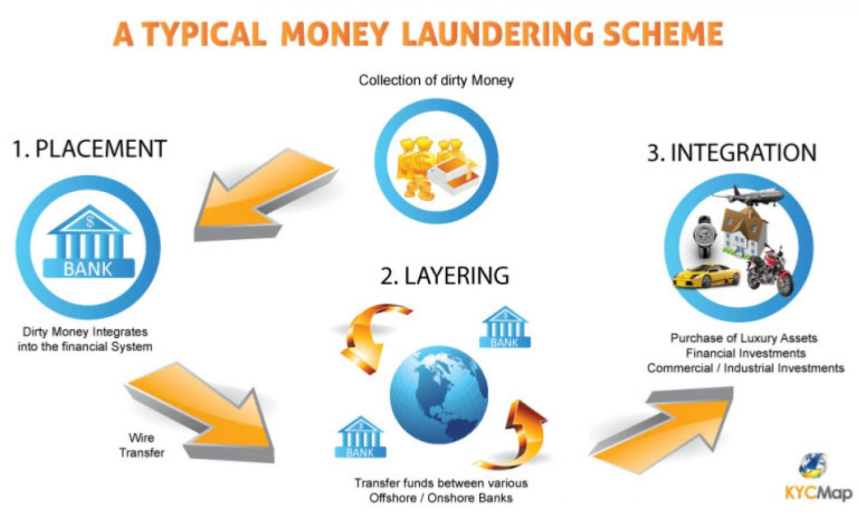
\includegraphics[width=0.85\textwidth]{slide_resources/money_laundering_cycle.png}
				\label{fig:money_laundering_cycle}
			\end{center}
		\end{figure}
	\end{frame}

%-------------------------------------------------------------------------------
	\subsection{Anti Money Laundering Current Design}
%-------------------------------------------------------------------------------
	\begin{frame}
		\frametitle{Anti Money Laundering}
		How are we solving Anti Money Laundering up until now?\\
		\begin{enumerate}
			\item We use Rule-Based systems that detect instances of money laundering.
		\end{enumerate}
		
		What are these rule-based systems?
		\begin{enumerate}
			\item FICO
			\item fiserv
			\item SAS AML
			\item Actimize
		\end{enumerate}
	\end{frame}

%-------------------------------------------------------------------------------
	\subsection{Anti Money Laundering Current Design}
%-------------------------------------------------------------------------------
	\begin{frame}
		\frametitle{Anti Money Laundering}

		If rule-based systems are solving Money Laundering then what remains to be a problem?\\
		\begin{enumerate}
			\item Process is manual
			\item Human intervention required at many steps
			\item Alerts have a high false positive rate - 75\% to 99\%
			\item The Rule-Based systems are slow to evolve. 
			\item Rule gaps, and complexities exist. 
			\item Rules are stratified, evolution of new rules requires \textit{only} AML systems to design these rules. 
		\end{enumerate}
	\end{frame}

%-------------------------------------------------------------------------------
		\subsection{Anti Money Laundering}
%-------------------------------------------------------------------------------
	\begin{frame}
		\frametitle{Current Work Flow}
		\begin{figure}[htb]
			\begin{center}
				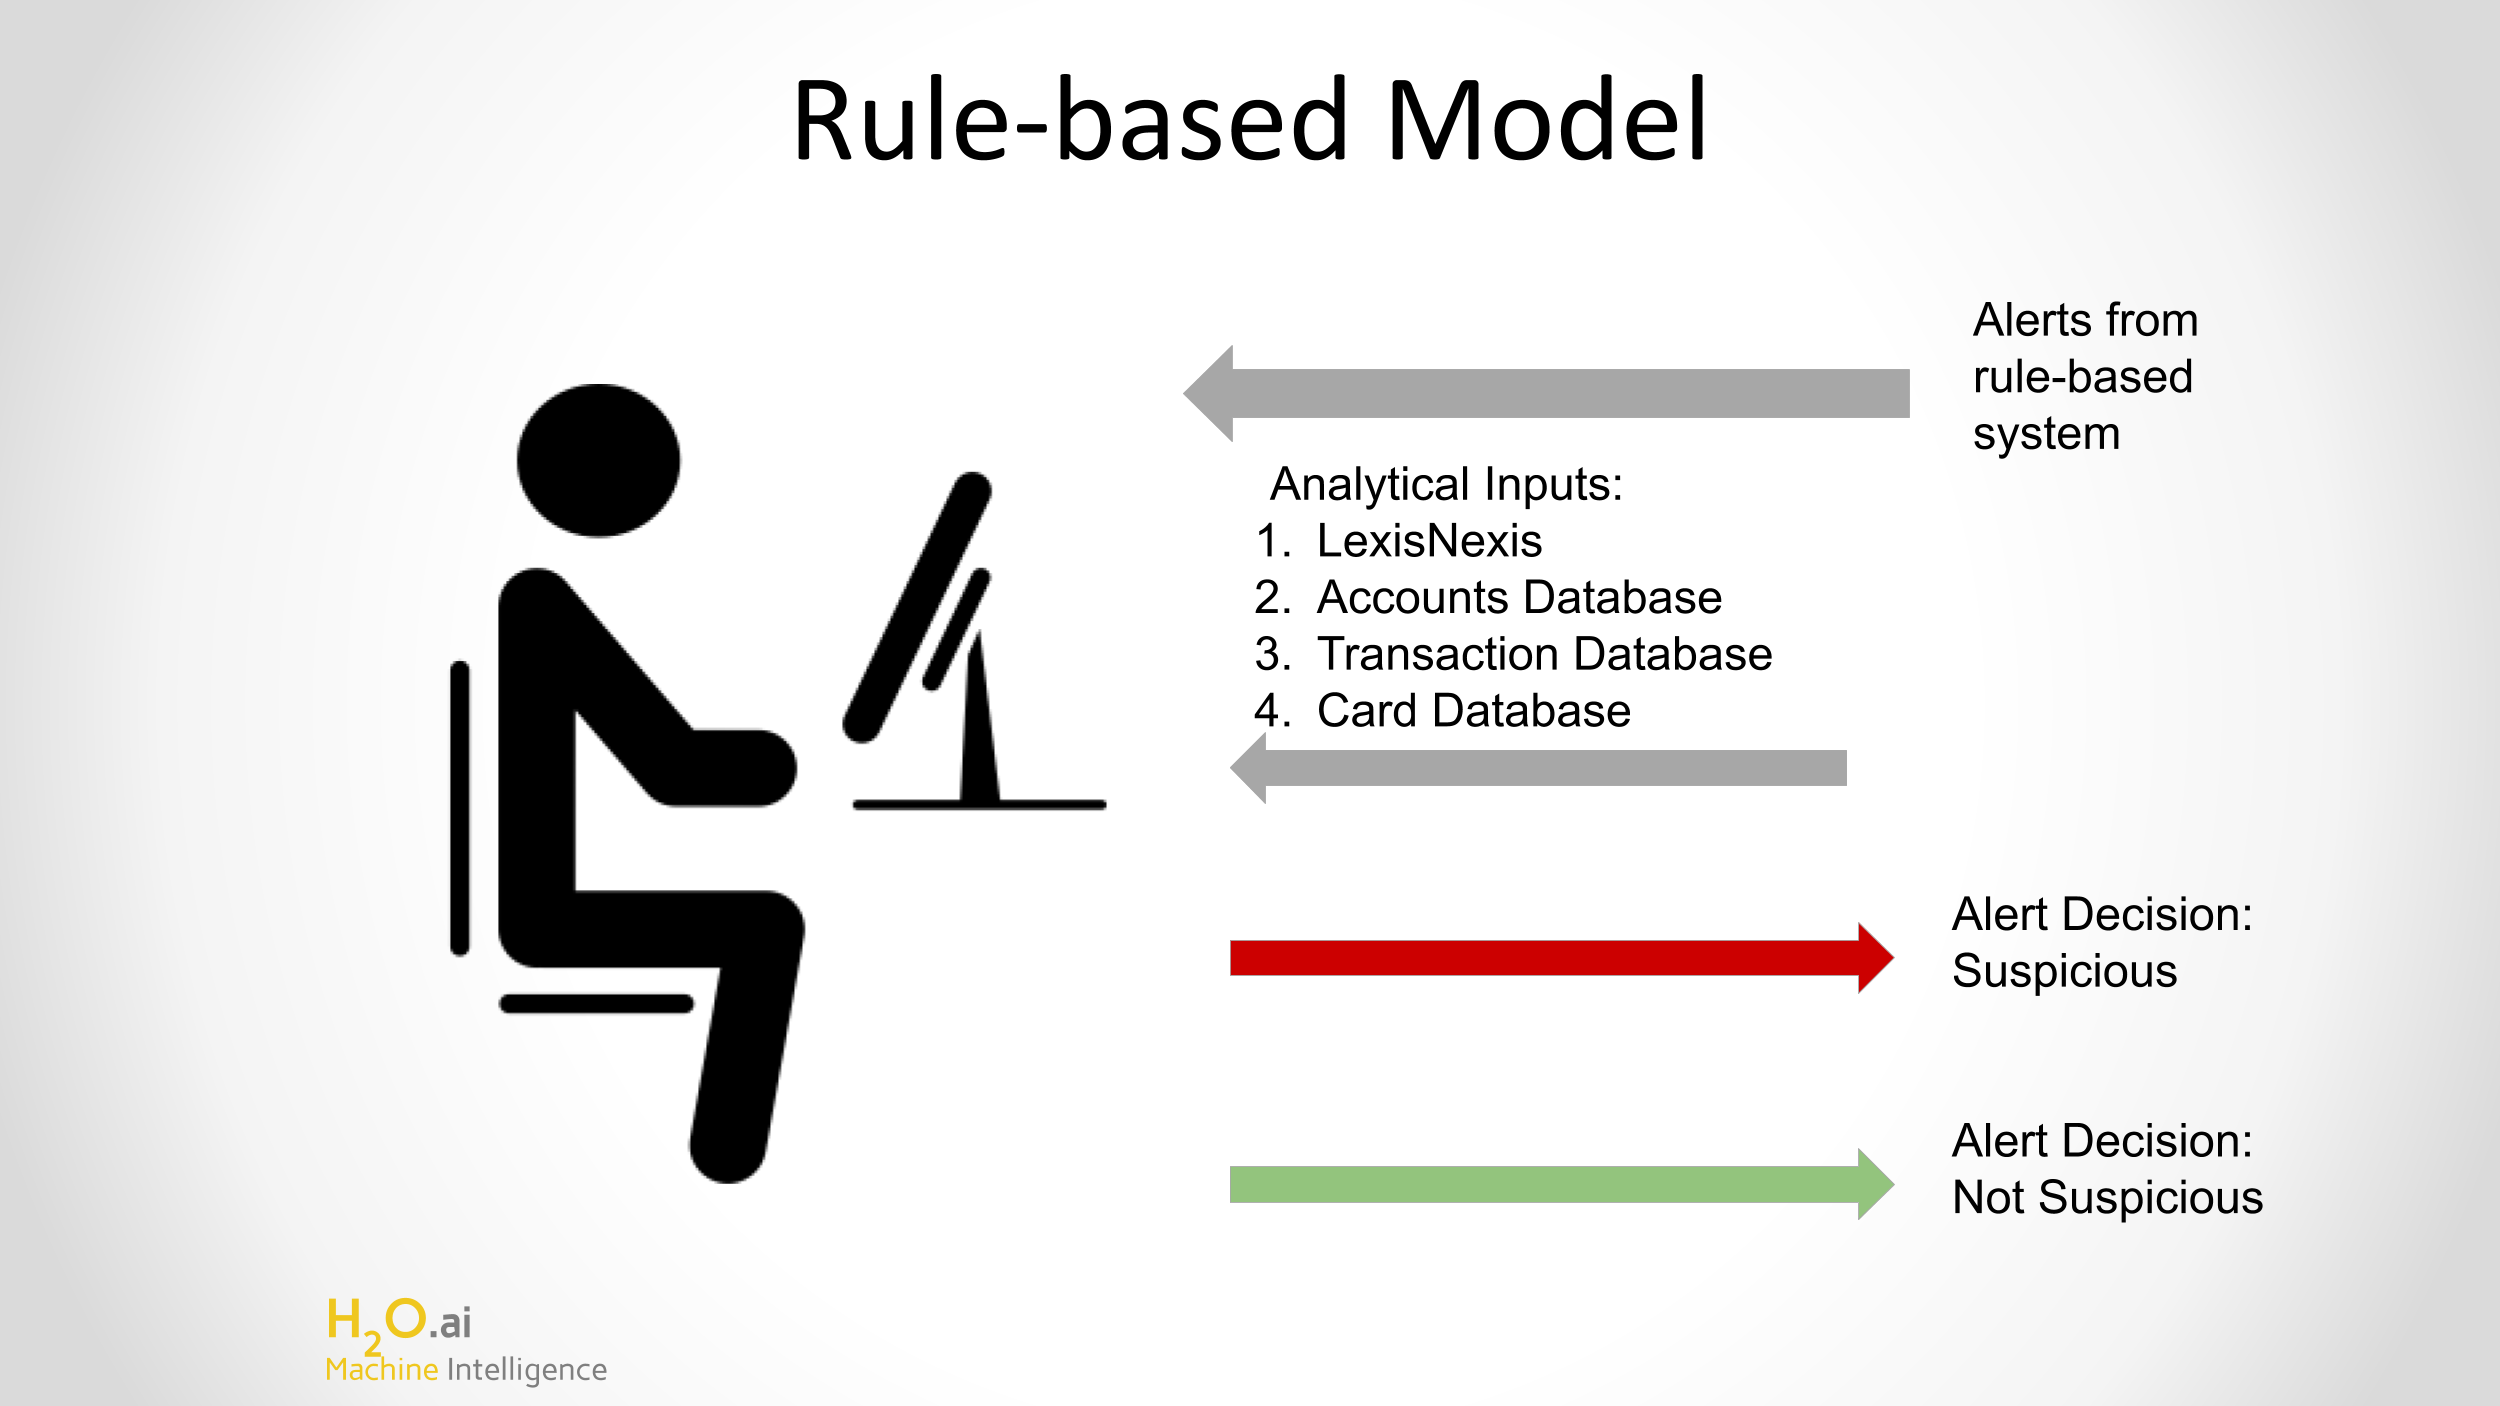
\includegraphics[width=0.85\textwidth]{slide_resources/Berlin-Meetup-AML.png}
				\label{fig:workflow}
			\end{center}
		\end{figure}
	\end{frame}
%-------------------------------------------------------------------------------
		\subsection{Anti Money Laundering}
%-------------------------------------------------------------------------------
	\begin{frame}
		\frametitle{Current Work Flow}
		The steps in the current rule-based workflow are:\\
		\begin{enumerate}
			\item An alert is generated by the alerting system (mostly false positive - 75\% to 99\%)
			\item The investigator reviews it.
			\item The alert is approved as True Positive, or classified as False Positive
		\end{enumerate}
	\end{frame}

%-------------------------------------------------------------------------------
		\subsection{Anti Money Laundering}
%-------------------------------------------------------------------------------
	\begin{frame}
		\frametitle{What Does the Anti-Money Laundering Solution Do?}
		
		\begin{enumerate}
			\item Fundamentally, it reduces false positives.
			\item The solution is strategically placed between the AML system and the investigator. 
			\item It classifies alerts as False Positive, or True Positive, using an out-of-loop ML approach.
			\item A curated set of alerts are given to the investigator. 
		\end{enumerate}
	\end{frame}

%-------------------------------------------------------------------------------
		\subsection{Anti Money Laundering}
%-------------------------------------------------------------------------------
	\begin{frame}
		\frametitle{What are the advantage of the AML Solution?}
		
		\begin{enumerate}
			\item Speed and Speed - Usual investigation time is about 45 - 90 days. The solution cuts it down to seconds. 
			\item It reduce human inaccuracies. 
			\item It reduce required person-hours. 
			\item It fills rule-gaps by innovative features. 
		\end{enumerate}
	\end{frame}

%-------------------------------------------------------------------------------
		\subsection{Anti Money Laundering}
%-------------------------------------------------------------------------------
	\begin{frame}
		\frametitle{What is the \textit{basic} modeling requirement to successfully use the AML Solution?}
		
		\begin{enumerate}
			\item The AML Solution requires the problem to be defined as a \textit{Supervised Machine Learning problem.}
			\item Therefore for training a model, the Solution requires historic alerts to be pre-marked as False Positives, or as True Positives, by the investigators.
		\end{enumerate}
	\end{frame}

%-------------------------------------------------------------------------------
		\subsection{Anti Money Laundering}
%-------------------------------------------------------------------------------
	\begin{frame}
		\frametitle{What are the data sources required by the AML Solution?}
		
		\begin{enumerate}
			\item Pre-marked AML Alert Data
			\item Banking Transactional Data
			\item Banking KYC (customer) data
		\end{enumerate}
	\end{frame}

%-------------------------------------------------------------------------------
	\section{Questions}
%------------------------------------------------------------------------------

		\begin{frame}

			\frametitle{Demo}

		\end{frame}
%-------------------------------------------------------------------------------
		\subsection{Anti Money Laundering}
%-------------------------------------------------------------------------------
	\begin{frame}
		\frametitle{How is the AML Solution deployed?}
		
		\begin{enumerate}
			\item The AML Solution does not modify any \textbf{\textit{existing}} AML alert generating system. 
			\item FIs invest considerable resources around Rule-Based AML alert generators, and replacing them with a complete ML-Based solution is slow. Therefore the AML Solution works around these Rule-Based alert generators. 
			\item The AML Solution ingests Alerts from the database table (or a copy of,)  that the AML alert generating system writes to (e.g. SAS). 
			\item It then applies the AML specific feature transformations and creates a ML-Based model using DriverlessAI.
			\item Using the ML-Based model, alerts generated by the Rule-Based AML alert generating systems are classified as True Positve, or False Positive. 
			\item This classification is written back to the database for further investigation or to create a Suspicious Activity Report.
		\end{enumerate}
	\end{frame}

%-------------------------------------------------------------------------------
		\subsection{Anti Money Laundering}
%-------------------------------------------------------------------------------
	\begin{frame}
		\frametitle{Things to Remember}
		
		\begin{enumerate}
			\item The ability of the model is dependent on the risk appetite, which is dependent on the False Negative percentage. 
			\item High risk appetite can give better False Positive and True Positive classification, but will also increase the False Negatives. 
			\item The ability of the model will also depend on the quality and size of the data. 
		\end{enumerate}
	\end{frame}

%-------------------------------------------------------------------------------
	\section{Questions}
%------------------------------------------------------------------------------

		\begin{frame}

			\frametitle{Thank you \& Questions}

		\end{frame}


\end{document}
\end{document}
